\chapter{Iteracion 2: Primer prototipo de software} % (fold)
\label{cha:iteracion_2}

\section{Introduccion} % (fold)
\label{sec:introduccion}

% fue cuando empezamos a tirar fruta. habiendo elegido el microcontrolador empezamos a probar todas las funcionalidades: El adc, los contadores de eventos, el modulo serial. Despues arrancamos a diseñar el primer prototipo. Consideramos que segun los requerimientos tenia que se un sistema que ofrezca algun tipo de interfaz para que un usuario interactue con el, para que pueda configurarle los parametros segun lo que se quiere lograr.

En esta iteracion se realizo el primer prototipo de programa a embeber en el microcontrolador para cumplir con los requerimientos planteados. Los primeros pasos incluyeron programas de prueba para verificar el funcionamiento de los distintos modulos del microcontrolador a utilizar: El conversor analogico-digital, la ganancia programable, los contadores y el modulo serial. 

% section introduccion (end)

\section{Requerimientos de la iteración} % (fold)
\label{sec:requerimientos_de_la_iteracion}

De los requerimientos principales, surgen los siguientes requerimientos para el programa a embeber en el microcontrolador:

\begin{itemize}
\item El programa deberia utilizar el conversor del microcontrolador para transformar señales analogicas de fuentes externas a datos digitales
\item El programa deberia utilizar los contadores del microcontrolador para contar eventos de fuentes externas
\item El programa deberia utilizar el modulo serial UART y SMBus del microcontrolador para enviar los datos a otra placa o microprocesador
\item Para cada canal del conversor:
\begin{itemize}
\item El usuario deberia poder habilitar o inhabilitar el canal para la medicion
\item El usuario deberia poder configurar el modo de medicion (canal unico o diferencial). En caso de ser canal unico deberia especificarse un solo canal, y dos canales para modo diferencial.
\item El usuario deberia poder configurar un tiempo entre cada medicion
\end{itemize}
\item Para cada contador:
\begin{itemize}
\item El usuario deberia poder habilitar o inhabilitar el conteo de eventos.
\end{itemize}
\item El usuario deberia poder elegir el protocolo serial para comunicarse con la placa o microprocesador externo que recibira los datos (UART o SMBus).

\end{itemize}


% section requerimientos_de_la_iteracion (end)

\section{Desarrollo} % (fold)
\label{sec:desarrollo}

En esta seccion elaboramos el proceso de desarrollo que se llevo a cabo para construir el software a embeber en el microcontrolador C8051F252\cite{c8051f352}. Es necesario que se tenga en cuenta que fueron necesarias dos iteraciones para llegar al prototipo final. En esta seccion cubrimos solo la primera. La segunda iteracion de software, que fue en la que se llego al programa final de la placa de adquisicion, se encuentra en el capitulo \ref{cha:iteracion_4}

\section{Diseño y modelos estaticos} % (fold)
\label{sec:diseno_y_modelos_estaticos}

Para poder describir el programa de manera grafica, utilizamos modelos del patron de diseño SysML 1.1. Aunque no usamos este patron de diseño para el programa, lo utilizamos en este informe para describirlo de una manera formal.

\subsection{Modelos estaticos} % (fold)
\label{sub:modelos_estaticos}

Como primera instancia, realizamos un diagrama de caso de uso para tener una idea de lo que se quiere lograr con el programa. Es necesario tener en cuenta que por las caracteristicas del microcontrolador, existen ciertas limitaciones que limitan el software. Estas limitaciones estan listadas en la seccion \ref{sub:seleccion}.

\begin{figure}[h]
  \centering
  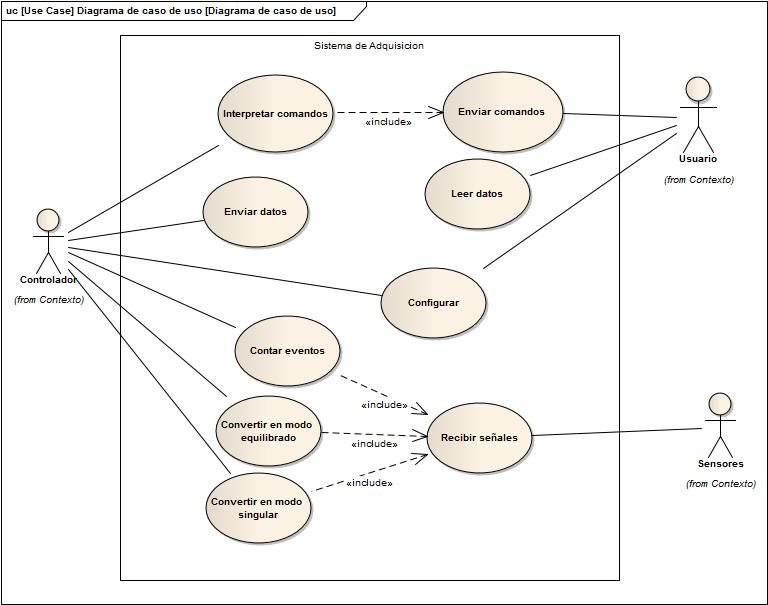
\includegraphics[width=0.80\textwidth, height = 11cm]{casouso1}
  \caption{Diagrama de caso de uso del sistema de medicion e instrumentacion}\label{fig:casouso1}
\end{figure}

El caso de uso ``configurar'' esta generalizado. Las acciones que incluye este caso son:
\begin{itemize}
	\item Configurar la interfaz serial
	\item Configurar canal en modo singular
	\item Configurar canal en modo equilibrado
	\item Configurar contador de eventos
	\item Configurar ganancia del del conversor
	\item Configurar intervalo de medicion para conversion analogica
\end{itemize}

\begin{figure}[h]
  \centering
  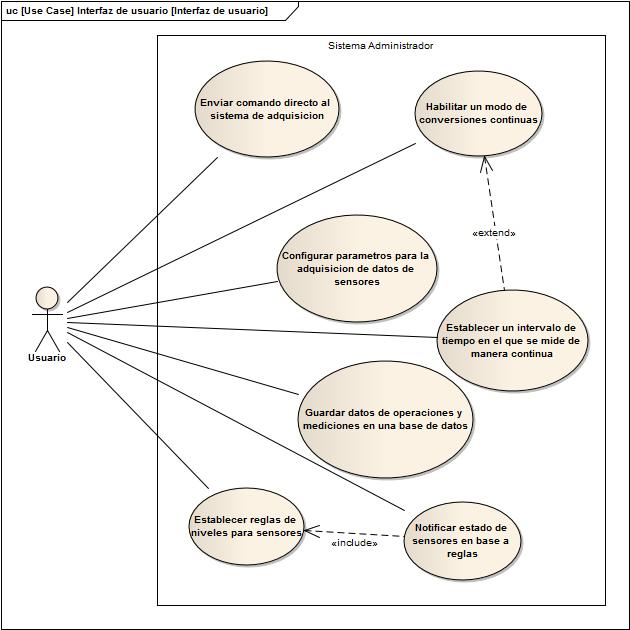
\includegraphics[width=0.80\textwidth, height = 11cm]{casousoAdministrador}
  \caption{Diagrama de caso de uso del sistema administrador}\label{fig:casousoAdministrador}
\end{figure}

En la figura \ref{fig:casouso1}, se puede ver el diagrama de caso de uso para el software a realizar. En cada caso de uso, pueden comenzar a visualizarse las distintas acciones que el programa debe realizar. Al no contar con la posibilidad de organizar el programa en clases, se separo en distintos modulos que agrupan funciones de caracteristicas similares. Estos modulos estan ilustrados como bloques en la figura \ref{fig:bloquesprimeraiteracionsoftware}. Cada bloque correponde a un modulo distinto dentro del programa. Se pueden ver los nombres de cada funcion y el tipo de retorno en cada uno de ellos. Con esto ultimo, damos una idea de las acciones realizadas por las funciones de cada modulo. Una descripcion mas detallada esta en la documentacion del programa \ref{documentacionsoftware}. 

\begin{figure}[h]
  \centering
  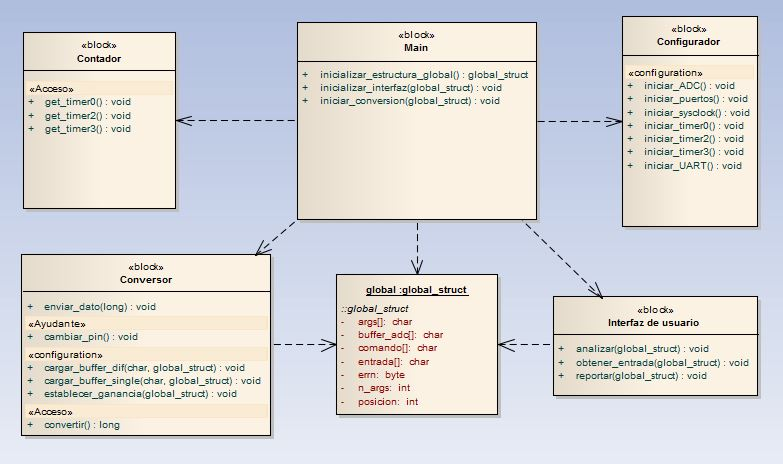
\includegraphics[width=0.80\textwidth, height = 11cm]{bloquesprimeraiteracionsoftware}
  \caption{Diagrama de bloques de la primera iteracion de software}\label{fig:bloquesprimeraiteracionsoftware}
\end{figure}

% subsection modelos_estaticos (end)


% section diseño_y_modelos_estaticos (end)
% section desarrollo (end)

\section{Pruebas} % (fold)
\label{sec:pruebas}

% section pruebas (end)

\section{Resultados} % (fold)
\label{sec:resultados}

% section resultados (end)

% chapter iteracion_3 (end)